\PassOptionsToPackage{unicode=true}{hyperref} % options for packages loaded elsewhere
\PassOptionsToPackage{hyphens}{url}
%

\documentclass[1p]{elsarticle}
%\documentclass[12pt,review,3p,authoryear,longnamesfirst]{elsarticle}

\usepackage{lmodern}
\usepackage{amssymb,amsmath}

  \usepackage[T1]{fontenc}
  \usepackage[utf8]{inputenc}
  \usepackage{textcomp} % provides euro and other symbols

% use microtype if available
\IfFileExists{microtype.sty}{%
\usepackage[]{microtype}
\UseMicrotypeSet[protrusion]{basicmath} % disable protrusion for tt fonts
}{}

\usepackage{hyperref}
\hypersetup{
            pdfborder={0 0 0},
            breaklinks=true}
\urlstyle{same}  % don't use monospace font for urls
\usepackage{longtable,booktabs}
% Fix footnotes in tables (requires footnote package)
\usepackage{graphicx,grffile}
\makeatletter

\makeatother

\date{}

%Some macros by BB
\usepackage{color}
\usepackage{soul}
\usepackage{multirow}
\usepackage{rotating}
%\usepackage{ulem} % crossed text
\definecolor{turquoise}{cmyk}{0.65,0,0.1,0.1}
\definecolor{purple}{rgb}{0.65,0,0.65}
\definecolor{darkgreen}{rgb}{0.0, 0.5, 0.0}
\definecolor{darkred}{rgb}{0.5, 0.0, 0.0}
\definecolor{darkblue}{rgb}{0.0, 0.0, 0.5}
\definecolor{blue}{rgb}{0.0, 0.0, 1.0}

\newcommand{\egfinal}[1]{{#1}}
%\newcommand{\changed}[1]{{#1}}
\newcommand{\changed}[1]{{\color{red}[{#1}]}}
\newcommand{\tog}[1]{{#1}}
\newcommand{\togerase}[1]{\st{#1}}

\newcommand{\qa}[2]{\marginpar{\color{red}\textbf{A\,#1}}{\color{red}#2}}
\newcommand{\todo}[1]{\textbf{ \color{red}[todo: #1]}}
\newcommand{\erase}[1]{\st{#1}}
\newcommand{\del}[1]{\st{#1}}
\newcommand{\BB}[1]{{\textbf{ \color{cyan}[BB: #1]}}}
\newcommand{\bb}[1]{{\textbf{ \color{cyan}[BB: #1]}}}
\newcommand{\sk}[1]{{\textbf{ \color{red}[SK: #1]}}}
\newcommand{\THCOMMENT}[1]{{\bf \color{magenta}[TH: #1]}}
\newcommand{\rep}[2]{\textbf{ \color{cyan}[replace: #1 {\it with} #2]}}
\newcommand{\ale}[1]{\textbf{ \color{green}[Ale: #1]}}
\newcommand{\ALE}[1]{\textbf{ \color{green}[Ale: #1]}}
\newcommand{\PF}[1]{\textbf{ \color{green}[PF: #1]}}
\newcommand{\pf}[1]{\textbf{ \color{green}[PF: #1]}}
\newcommand{\SP}[1]{\textbf{ \color{red}[SP: #1]}}
\newcommand{\meta}[1]{{\color{blue}[meta: #1]}}
\newcommand{\hide}[1]{{}}
\newcommand{\mbf}[1]{\mathbf{#1}}
\newcommand{\ch}[1]{{#1}}
\newcommand{\eg}{{\textit{e.g., }}}
\newcommand{\ie}{{\textit{i.e., }}}
\newcommand{\etal}{{\textit{et al.}}}
%end of some macros by BB

%\usepackage{natbib}
%\bibliographystyle{unsrtnat}
\bibliographystyle{elsarticle-harv}

\begin{document}
\begin{frontmatter}


\title{An Algorithm for Automatic Dormant Tree Pruning }

\author[FERI]{Simon Kolmani\v{c}}\corref{CoresAuth}\ead{simon.kolmanic@um.si}
\author[FERI]{Damjan Strnad}
\author[FERI]{\v{S}tefan Kohek}
\author[PURDUE]{Bedrich Benes}
\author[PURDUE]{\newline Peter Hirst}
\author[FERI]{Borut \v{Z}alik}

\address[FERI]{University of Maribor, Koro\v{s}ka cesta 46, 2000 Maribor, Slovenia}
\address[PURDUE]{Purdue University, West Lafayette, IN 47906, USA}

\begin{abstract}
Tree pruning is a labor and cost intensive task, but it is a necessary
measure that ensures high yield of good quality in horticulture and increases the overall health of trees in general. However, a great deal of experience is necessary in order to correctly prune a tree without causing series damage to it.
Extensive research has been made on how to automate the pruning
procedure and what is the actual effect of pruning on trees. 

We introduce a two-step method for automatic tree pruning that simulates pruning by detecting branches that should be removed in order to optimize a virtual tree light intake. Our two step algorithm starts by trimming the tree into a desired initial shape. In the second step a discrete differential evolution method is used to optimize the light distribution within the tree crown by detecting branches that should be trimmed, and virtually removing them. Our algorithm does not use a predefined set of pruning rules. Instead, it is an automatic optimization driven by the discrete differential evolution algorithm. We demonstrate our method by simulating the pruning of virtual trees in the EduAPPLE system by proposed algorithm and a human expert and compared the results. Our comparison shows that our algorithm selects branches similarly to human experts. The trees can also be formed into various growing forms, depending on the initial shape used. We believe that our algorithm is an important step towards pruning task automation.
\end{abstract} 

\begin{keyword}
Computer Graphics \sep Virtual Tree  \sep Tree Pruning \sep Pruning Automation \sep Discrete Differential Evolution\sep Tree Height Control
\end{keyword}

\end{frontmatter}

\section{Introduction}
Tree pruning is the process of removing branches usually with the main
objective of allowing more light in the canopy. Old and dead branches are
removed as well as living ones to balance the reproductive and
vegetative growth in the fruit production. Pruning must be done carefully not to damage the tree, to prevent fungus infections on the cuts, and not to damage the tree in general. This makes pruning one of the most expensive and labor-intensive tasks that is responsible for approximately 20\% of the annual pre-harvest cost for crops like apples, cherries, and pears~\cite{karkee_identification_2014}. A large crew of trained seasonal workers is needed to accomplish this task each winter, following a set of predefined rules~\cite{akbar_novel_2016}. 

Extensive research has been done on how to automate the tree pruning process in order to reduce costs and/or demands for the skilled workforce~\cite{jensen_effects_1980,karkee_identification_2014,moore_mechanical_1958}
on mass pruning by maintaining the specified distance from the tree
canopy center with limited ability to ensure a high pruning quality. The
fully automated results were not satisfying, as evidenced by the reduced quality and
yield of fruit~\cite{karkee_identification_2014}. 
Another previous work used mobile platform for automated pruning of grape vines~\cite{botterill_robot_2017}. 
Although the tree structure is more complex that those of
grape vines, the essence of the approach to the pruning automation is
similar. Both approaches create a 3D model of the plant by using computer vision
that recognized the tree structure and a decision system determines which
parts of the plant should be removed. Actual pruning is carried out by a six degree-of-freedom
robotic arm. Both, the apple tree and vine pruning are carried out while
the plants are in a dormant state, and in both cases, a set of
predefined pruning rules controls the pruning.

One of the bottlenecks of the current models is the 3D tree model
reconstruction. Plant reconstruction is an open problem by itself
and many approaches have been introduced~\cite{livny_automatic_2010,xie_tree_2016,zhang_data-driven_2014}. 
By applying the tree pruning rules on the generated tree 3D model the
surplus branches are identified that have to be removed~\cite{akbar_novel_2016,elfiky_automation_2015,medeiros_modeling_2017}.
As in pruning in general, these rules aim to increase the irradiance intake of the canopy,  to improve the tree health~\cite{simon_does_2006} and, in effect, fruit quality~\cite{bastias_light_2012}. 
%The overall fruit quality is additionally enhanced by removing weak shoots, and thus controlling the tree size. \sk{It is true that the removing of weak shoots improves the fruit quality but tree size is not directly important for the yield quality. It is important however for easier manipulation of trees and protection against hail by kipping the tree under the hail nets} 

One of the main problems of the previous work is that the trees are
removed by using fixed rules. The key observation of our work is
that we can generate the rules for each plant individually by using mathematical optimization.
In this paper, we propose an alternative
to the fixed set of pruning rules, by introducing a new two-step
procedure, which combines the pruning approach of the first mechanical
pruning systems with the selective pruning. In the first step, the tree
is trimmed according to a predefined template to maintain a desired
tree height and the distance to its neighbors. The first step attempts to minimize mutual tree shading, bud drying by their abrasion, and mutual tree competition.
In the second step, a mathematical optimization algorithm is used to determine which branch should be removed. Although many options exist, we use 
the discrete differential evolution (DDE)~\cite{strnad_novel_2017}. 

We have implemented our method in a software apple tree plant simulator EduAPPLE~\cite{kohek_eduapple:_2015}. We run several experiments,
where we used two different pruning templates in the first
step of pruning, a cylinder and a cone. 
We compared the light distribution inside the tree crown after pruning trees using the
newly-developed method with those pruned by the expert.
Our results show comparable levels of irradiance withing the canopy.
Moreover, by using the proposed pruning method for several consecutive
years, \bb{the trees avoid competing with their branches for the shared areas,} along
with their height, which is essential in high-density orchards.

\section{Materials and Methods}

In the proposed approach to automated tree pruning, a predetermined set
of tree pruning rules is replaced by an objective function which
includes the goals that have to be achieved by the pruning, combined
with the pre-pruning of a tree to cylindrical/conical shape. For the
sake of this experiment, the objective function prefers the maximization
of received light in the tree crown. For the optimization of the
objective function, discrete differential evolution method is used,
closely connected to a virtual tree model \cite{kohek_eduapple:_2015}, which is based on the
concept of self-organization \cite{palubicki_self-organizing_2009}.

\subsection{Tree Growth Model}

A tree model used in our approach is represented as a hierarchy of
modules as shown in Fig.~\ref{fig:my_figure1}~a) that is a common approach used in many plant
simulators such as \cite{de_reffye_plant_1988,palubicki_self-organizing_2009,pirk_plastic_2012,prusinkiewicz_development_1988,stava_inverse_2014}. The point at which one or more
leaves are attached to the stem is called a node. The part of the stem
between two nodes is an internode. The growth is controlled by apical
meristem that is a region of dividing cells that responds to gravity and
to the incoming light. In this way the tree grows against gravity
(gravitropism) and seeks the light (phototropism). Depending on the
plant DNA and environmental factors (light, temperature, nutrients) the
plant produces lateral buds that are either dormant or active. An
internode with attached leaves and lateral bud is called a metamer and a
sequence of metamers created at single spurt forms a shoot. The shoot
axis is produced by the terminal bud which is located at the end of the
shoot.

Our approach uses the previously developed framework called EduAPPLE~\cite{kohek_eduapple:_2015},
where the tree growth is driven by buds' illuminations~\cite{benes_efficient_1996,benes_visual_1997,mech_visual_1996} and a competitive process for growth resources~\cite{alsweis_modeling_2005,arvo_modeling_1988,palubicki_self-organizing_2009,runions_modeling_2007}, which leads to the self-organizing structure of the tree. The
tree attempts to maximize its branch mass by growth and light intake by
growth. Buds with higher irradiance produce new shoots that fill the
empty space. Buds in lower irradiance produce quickly growing shoots
that attempt to get from shade. Poorly illuminated buds do not create
new shoots, become dormant, and can form new shoots later, when the
conditions are more favorable. The key factor of this simulation is the
calculation of the illumination of leaves that feed buds and several
algorithms exists. Although inner reflection can be considered \cite{soler_efficient_2003},
the algorithms are usually time consuming, and the indirect light does
not contribute significantly to growth, because major light intake is
given by the direct lighting. A faster way is to use only the direct
irradiance~\cite{benes_visual_1997,benes_efficient_1996,mech_visual_1996,pirk_plastic_2012}. 
The tree cast shadow on itself and thus
forming a shadow space of the tree as shown in Fig.~\ref{fig:my_figure1}~b). The shadow
density is highest at the trunk; thus no leaves/shoots can grow from the
dormant buds positioned there. The key contribution of pruning is in
improving the illumination of the inner parts of the tree. When the
lighting conditions around the stem improve after removing some
branches, dormant buds can reactivate and start to produce new shoots.
\begin{figure}[hbt]
    \centering
    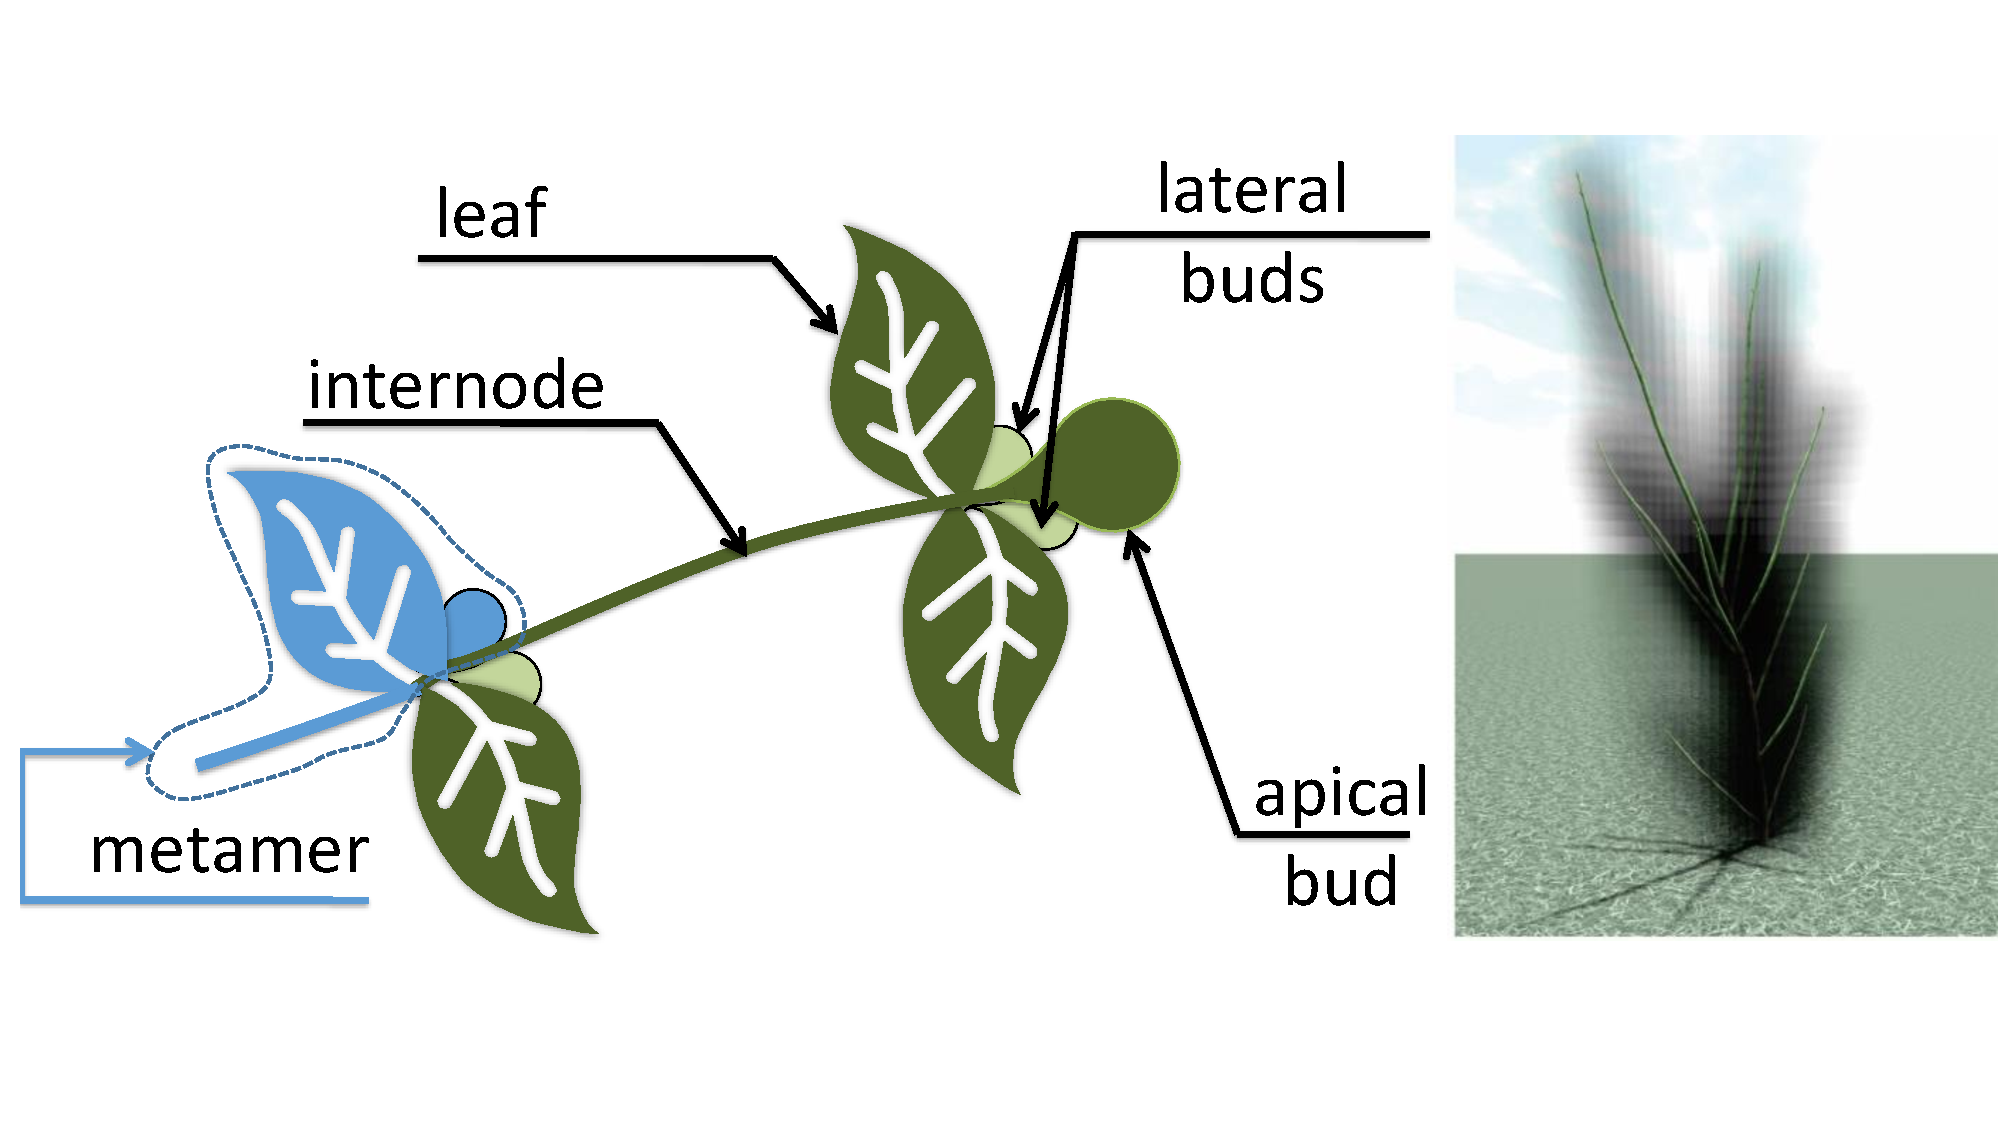
\includegraphics[width=4.5in]{figs/Fig1}
    \caption{a) Plant modules of a self-organizing tree growth
model, b) shadow space of a tree in used tree growth model from \cite{kohek_eduapple:_2015}.}
    \label{fig:my_figure1}
\end{figure}


\subsection{Illumination}

We calculated the inner shading by using the algorithm from \cite{palubicki_self-organizing_2009}
that was later extended in~\cite{pirk_plastic_2012,stava_inverse_2014,strnad_novel_2017}. The light distribution
inside the tree crown is calculated from the illuminated leaves that are
sources of a conical shadow volume. We calculate the bud illumination.
Suppose, we have a bud inside one of the shadow volumes of one of the
neighbors. Let \(d_{y}\) be the bud's vertical distance from the volume
apex and \(d_{x,z}\) its horizontal distance from the volume axis, then
the received shadow, originating from a given shadow volume is
calculated by \cite{strnad_novel_2017}:


\begin{equation}
\Delta s = \left\{ \begin{matrix}
\text{ab}^{- 0.8\left( d_{y} + d_{x,y} \right)}, & \mathrm{\text{if}}\ d_{x,y} < d_{y} \\
0, & \mathrm{otherwise} \\
\end{matrix}, \right.\    
\end{equation}
where \(a\) \textgreater{} 0 and \(b\)\textgreater{} 0 are model
parameters from \cite{palubicki_self-organizing_2009} and were set to \(a = 0.05\) and \(b = 2\).
Total irradiance of a given bud is then calculated by:
\begin{equation}
  Q = max\begin{Bmatrix}
1 - s, & 0 \\
\end{Bmatrix},  
\end{equation}
where \(s\) is the cumulative contribution of all shadow volumes,
captured by the given bud.

\subsection{Differential Evolution and Pruning}
Differential Evolution (DE) is a heuristic approach for minimizing
possibly nonlinear and non-differential continuous objective function.
Developed by Storm and Price \cite{storn_differential_1997}, the method aims to optimize
certain properties of a system pertinently choosing the system
parameters, usually represented as a vector. Objective function models
the objectives while incorporating potential constraints. DE employs
evolutionary operators like mutation, crossover, and selection.

Discrete DE (DDE) variants have been presented in relation to specific
combinatorial optimization problems, e.g., \cite{davendra_flow_2009,pan_discrete_2008,wang_novel_2010}. The DDE has
been used for the optimization of light condition inside the tree crown
by removing certain branches in \cite{strnad_novel_2017} in particular four optimization
methods have been used: BinDE, IndexDE, PathDE, and SetDE. Through
optimization of pruning locations, a combination of cuts is obtained
that maximizes the amount of light received by the remaining buds of the
tree crown. For that purpose, for all buds in the tree crown the
irradiance is calculated by the use of Eq. (2). Bud's irradiance, \(Q\)
corresponds to the percentage of available light intercepted by the bud.
For the sake of faster detection of ancestor/successor relationship
between internodes, each internode is associated with a unique
variable-length binary string as shown in~Fig.~\ref{fig:my_figure1}~b. Tree crown light
distribution is calculated next, where the irradiance of each bud in the
crown is assigned to one of ten quantization classes of equal width on
the interval {[}0, 1{]}. The objective function, \emph{f}(\textbf{x}),
is:
\begin{equation}
 f\left( \mathbf{x} \right) = \frac{\sqrt{S_{\mathrm{\text{tree}}}}}{H}\sum_{i = 1}^{10}{i \times h_{i}}, 
\end{equation}
where \(S_{\mathrm{\text{tree}}}\) is the number of remaining internodes
after pruning, \emph{H} is the total number of buds, and \(h_{i}\) is
the number of buds in the \emph{i}-th class of light distribution.

We define an optimization function that describes the light interception
of the tree as the sum of interception of all buds
\begin{equation}
   f\left( \mathbf{x} \right) = \sum_{i = 1}^{n}E_{i},
\end{equation}
where $n$ is the number of buds that remain after the pruning,
$E_{i}$ is the irradiance of the \(i\)-th bud. The function $f(\mathbf{x})$ is the total irradiance of the tree for a configuration \(x\) of the buds,
also called the solution vector. The solution vector is denoted by
\(\mathbf{x} = \ \left\{ x_{1},\ \ldots,x_{s} \right\}\) and it contains
the encoded sequence of cut positions, labeled by the corresponding
internodes. The root is denoted by a bit-string ``0''. A `0' or `1' is
appended to the parent's string for each main or lateral child
internode, respectively (Fig.~\ref{fig:my_figure1}~b). Each cut position \(x_{i}\)
identifies the internode, at which the branch is removed. Variable
\emph{s} in this case is a population size and is a value between
\(s_{\mathrm{\min}}\) and \(s_{\mathrm{\max}}\), which are custom set
parameters, representing the minimum and the maximum number of allowed
cuts. The objective function \(f(\mathbf{x})\) favors solutions that
provide a maximal improvement of light distribution with minimum amount
of removed biomass. It is very important to recognize a redundant cuts,
for example, if a cut should be made at internode ``00'', the cuts
``001'', ``000'', or ``0010'', would be redundant and thus unnecessary
as shown in Fig.~\ref{fig:my_figure2}. Our labeling allows for quick detection of the
redundant cuts. In a given example the later three internodes share the
same prefix ``00'', which is the label of their predecessor and with
removing it, all of its successors are removed as well.

\begin{figure}[hbt]
    \centering
    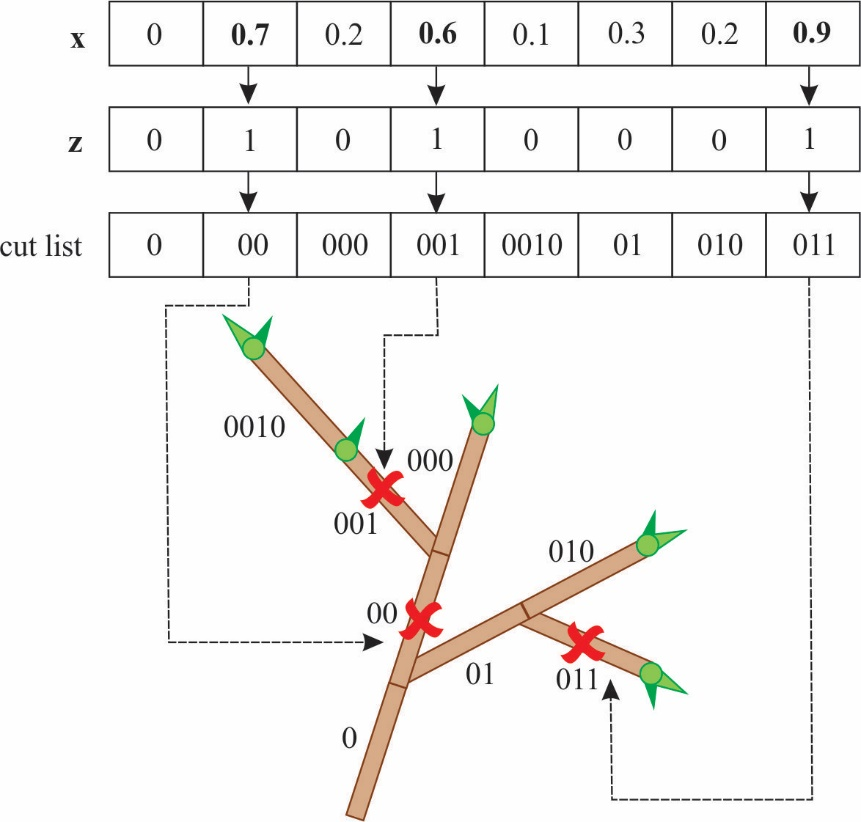
\includegraphics[width=3.3in]{figs/image2.jpeg}
    \caption{Mapping of the solution vertex into the tree cutting
sequence. Solution vector components that exceed the threshold are
converted into the cuts with the help of the cut list.}
    \label{fig:my_figure2}
\end{figure}


For our experiment, we have selected only BinDE optimization method
because the pruning results were visually close to those of the human
expert. The encoding scheme of BinDE uses the real-valued vectors to
represent solution genotypes. For the mapping of genotypes to pruning
instances, the intermediate cut list is used. It is produced by
traveling the tree model in a depth-first manner and recording the
labels of all internodes encountered in the process into a list. The
length of the cut list defines the dimensions of solution vectors. Each
component \(x_{i,j} \in \ \left\lbrack 0,\ 1 \right\rbrack\) of the
solution vector \(\mathbf{x}_{i}\ \)determines whether \emph{j}-th
internode from the cut list will be selected as the cutting point or
not. For that purpose the binary vector \(\mathbf{z}_{i}\) is
constructed by thresholding:
\begin{equation}
    z_{i,j} = \ \left\{ \begin{matrix}
0, & \mathrm{\text{if}}\ x_{i,j} < 0.5 \\
1, & \mathrm{\text{otherwise}} \\
\end{matrix}, \right.\
\end{equation}


If the number of cuts proposed by the vector \(\mathbf{z}_{i}\) violates
the solution size constraints, the threshold is adjusted up or down
until the constraints are met. The entire mapping operation is shown in
Fig.~\ref{fig:my_figure2}.

\subsection{Tree Height and Neighboring Distance Control}
Although the DDE method significantly improves the light conditions
inside the tree crown, it offers no control over the tree size or the
distance to neighbor trees. Since the modern orchards are mostly
protected by the anti-hail nets, it is crucial to keep apple trees at a
certain height. Similarly, the neighboring distance that, has to be
preserved during the entire lifetime of an orchard.

A straightforward method to get control over the tree height and
neighboring distance would be the extension of the objective function
\(f\left( \mathbf{x} \right)\) with additional constraints regarding the
tree size. It turned out, however, that while the integration of the
tree height into the tree model and objective function is possible, the
determination of the extent of the tree crown after the pruning was not
very efficient.

Our inspiration for the solution to this problem comes from observing a
human during manual pruning. Instead of just following the pruning
rules, the human pruner strives to shape the tree into one of the
well-defined growing forms. Those growing forms were developed over the
years by the experts and gave the best fruiting results under certain
growing conditions. In the high density orchards, the most common tree
forms are the Slender Spindle \cite{weber_optimizing_2000}, and more recent, the Tall
Spindle \cite{robinson_vision_2013}. While the first growing form is more conically shaped
the second resembles a cylinder. Tall spindle is very popular because it
is suitable for mechanical pruning and formation of the Fruiting Wall
\cite{robinson_vision_2013}.

Instead of changing the objective function, we propose adding a
preprocessing level to the DDE method. We call this step pre-pruning and
by adding this the desired form, the tree height and neighboring
distance can be controlled easily. We prune the trees to circular shapes
(cone and cylinder) with adjustable height and the base radius. After
the branches outside the chosen shape are trimmed off, the DDE method is
used to optimize the light condition inside the tree crown. The entire
tree pruning process is depicted in Fig.~\ref{fig:my_figure3}.
\begin{figure}[hbt]
    \centering
    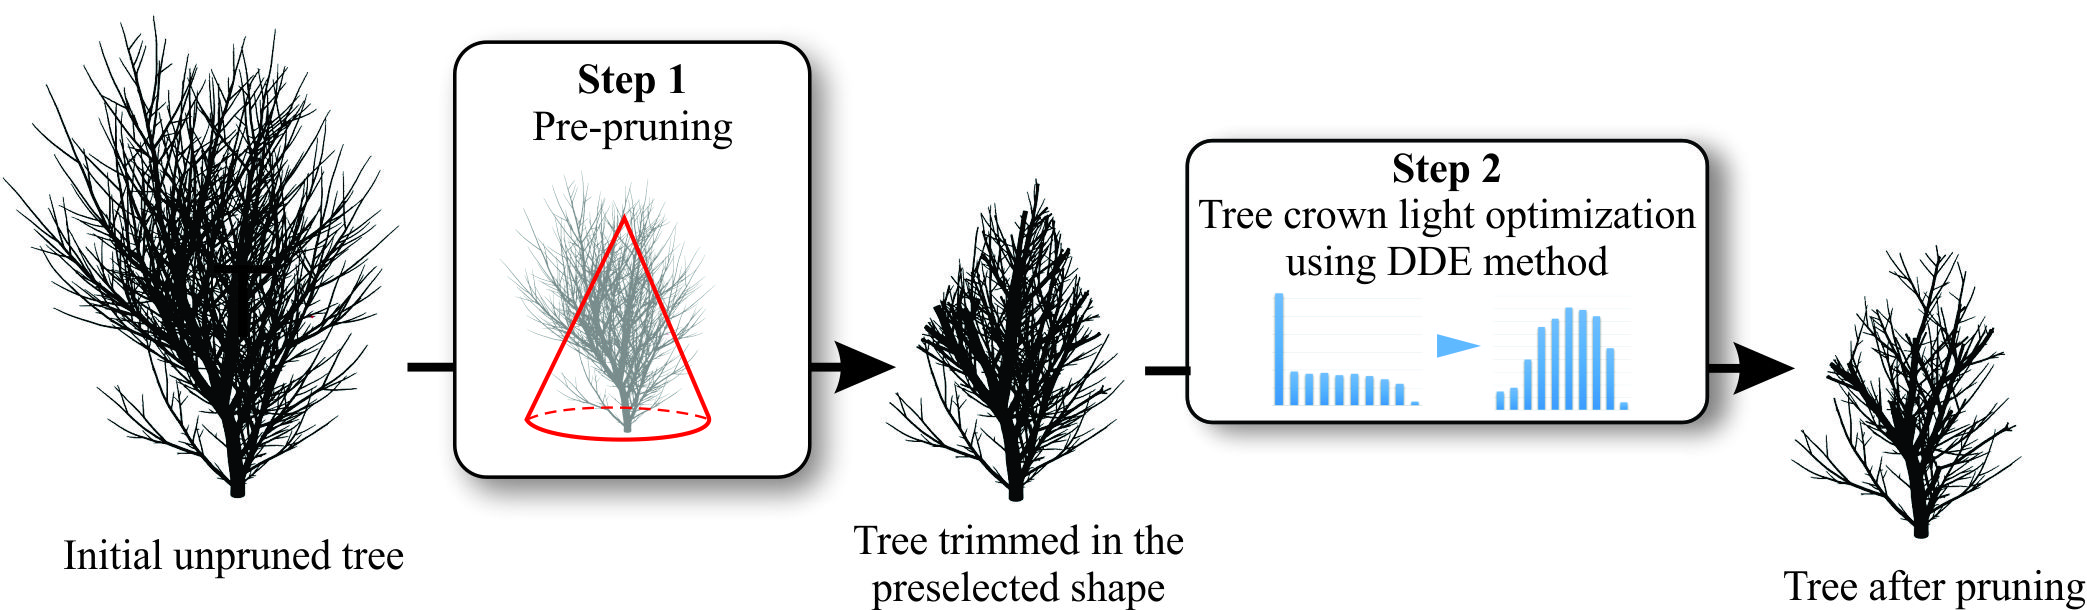
\includegraphics[width=5.3in]{figs/image3.jpeg}
    \caption{Two-step virtual pruning process enables the control
over tree height and neighboring distance. First, the tree is pre-pruned
into a cone or cylinder shape with adjustable size. In the second step
the DDE method selectively removes branches to improve the light
conditions inside the tree crown.}
    \label{fig:my_figure3}
\end{figure}

The results of the final pruning are highly dependent on the maximum
allowed number of cuts \(s_{\mathrm{\max}}\), which has to be adjusted
to the tree age and complexity of the tree crown. In our implementation,
we set \(s_{\mathrm{\max}} = 20\) which provided good results for young
trees. While we used circular proxies in our work, other shapes could be
used: for example, orchards with Fruiting Wall planting system could use
rectangular blocks.


\section{Results}
We pruned a four years old virtual
untrained tree (Fig.~\ref{fig:my_figure4}) by using the proposed method. The same tree was also pruned by horticulture expert and the results were compared.
The tree training teaching environment EduAPPLE~\cite{kohek_eduapple:_2015} was used for this purpose. The expert shaped the tree into two primary forms, a
pyramidal growing form (denoted as HeP -- Human expert - Pyramidal), which is similar to a Slender Spindle, and a
Flatt growing form (denoted as HeF -- Human expert - Flatt), suitable for the Fruiting Wall planting system. 
For the automated pruning, we used a cone with the height of \(3\)m and the
opening angle of \(45{^\circ}\) (denoted as DDECn -- DDE method, Conical initial shape), and a cylinder with a height of
3m and radius of 0.75 m (denoted as DDECy -- DDE method, Cylindrical initial shape). 
In both cases, we set \(s_{\mathrm{\max}}=50\). 
\begin{figure}[hbt]
    \centering
    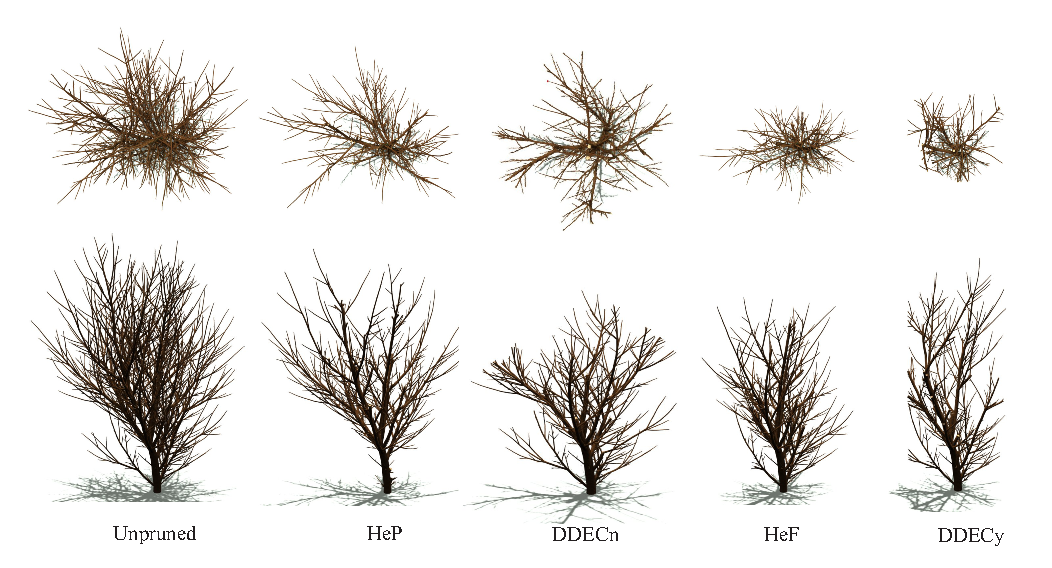
\includegraphics[width=\linewidth]{figs/Fig5.pdf}
    \caption{Comparison of pruning with the initial unpruned tree,
tree pruned by a human expert in a pyramidal shape (HeP), automated
pruning with initial cone shape (DDECn), pruning by human expert pruning
in a plat plane (HeF), automated pruning with the use of cylindrical
initial shape (DDECy).}
    \label{fig:my_figure4}
\end{figure}

\noindent\textbf{Light Distribution:} In all four cases, the light distribution inside the tree crown has
improved (see Table~\ref{tab:light}) as compared to the unpruned tree (Fig.~\ref{fig:my_figure5}) with the average increase of 168\% of buds. 
In particular, only 14.89 \% of buds receive more than 70 \% of available light in the unpruned trees, 
while in the the human-pruned tree the amount of such buds increases to 26.80 \% (HeP) and to the 22.95 \% (HeF).
The light distributions of the automated tree pruning are comparable with
that of human expert (25,93 \% for DDECn and 24.18 \% for DDECy). 
When comparing HeP to DDECn the result in the cases of human pruning is slightly better but in the case of HeF and DDECy the automated pruning achieved better result, although the difference in both casses is less than 1.3 \%.  
\begin{table}[hbt]
\label{tab:light}
\begin{center}
\begin{tabular}{ |l|c|c| } 
 \hline
 \textbf{Method} & \textbf{\% of buds receiving}                           & $\mathbf{\Delta}$ \textbf{to unpruned [\%]} \\ 
                 &  \textbf{more than 70\% of light}                       &  \\ 
 \hline
 \textbf{Unpruned}            & 14.89 & 0 \\ 
 \hline
 \textbf{Manual Expert (HeP)} & 26.80 & 180 \\ 
 \textbf{Manual Expert (HeF)} & 22.95 & 154 \\ 
  \hline
 \textbf{Automatic (DDECn)} & 25.93 & 174 \\ 
 \textbf{Automatic (DDECy)} & 24.18 & 162 \\ 
 \hline
\end{tabular}
\end{center}
\caption{The percentage of buds receiving more than 70\% of light in an unpruned tree and after manual pruning by using HeP and HeF methods and our automatic pruning by using DDECn and DDECy. The improvement in all cases is in average of 168\%. }
\end{table}

\noindent\textbf{Pruned Internodes:} The difference between the DDE and human pruning is also visible in the category of the internodes left in the tree after the pruning as shown in Table~\ref{tab:inodes}. The unpruned tree has 18,618 internodes. After manual pruning by using HeP the number decreased to 7,810 and manual pruning by using HeF decreased the number to 5,715. Automatic pruning provided smaller numbers. The DDECn algorithm pruned the tree to 5,714 and the DDECy to 4,867 nodes. The average number for manual pruning was 6,776 and for automatic 5,291.
\begin{table}[hbt]
\label{tab:inodes}
\begin{center}
\begin{tabular}{ |l|c|c| } 
 \hline
 \textbf{Method} & number of internodes on the tree  & $\Delta$ to unpruned [\%] \\ 
  \hline
 \textbf{Unpruned}            & 18,618 & 0 \\ 
 \hline
 \textbf{Manual Expert (HeP)} & 7,810 & 42 \\ 
 \textbf{Manual Expert (HeF)} & 5,715 & 31 \\ 
  \hline
 \textbf{Automatic (DDECn)} & 5,741 & 31 \\ 
 \textbf{Automatic (DDECy)} & 4,867 & 26 \\ 
 \hline
\end{tabular}
\caption{The number of internodes on the tree in an unpruned tree and the comparison to the number of internodes after manual pruning by using HeP and HeF methods and our automatic pruning by using DDECn and DDECy. The average number of internodes is 6,033 that corresponds to 32\% of nodes of the unpruned tree. }
\end{center}
\end{table}

By combining both results from Tables~\ref{tab:light} and~\ref{tab:inodes}, 
it can be concluded, that the human expert
achieved similar bud light exposure with less biomass removed,
which is desirable since the higher number of internodes with
well-illuminated buds represent the higher potential for the yield of
both increased quality and quantity. 

\begin{figure}[hbt]
    \centering
    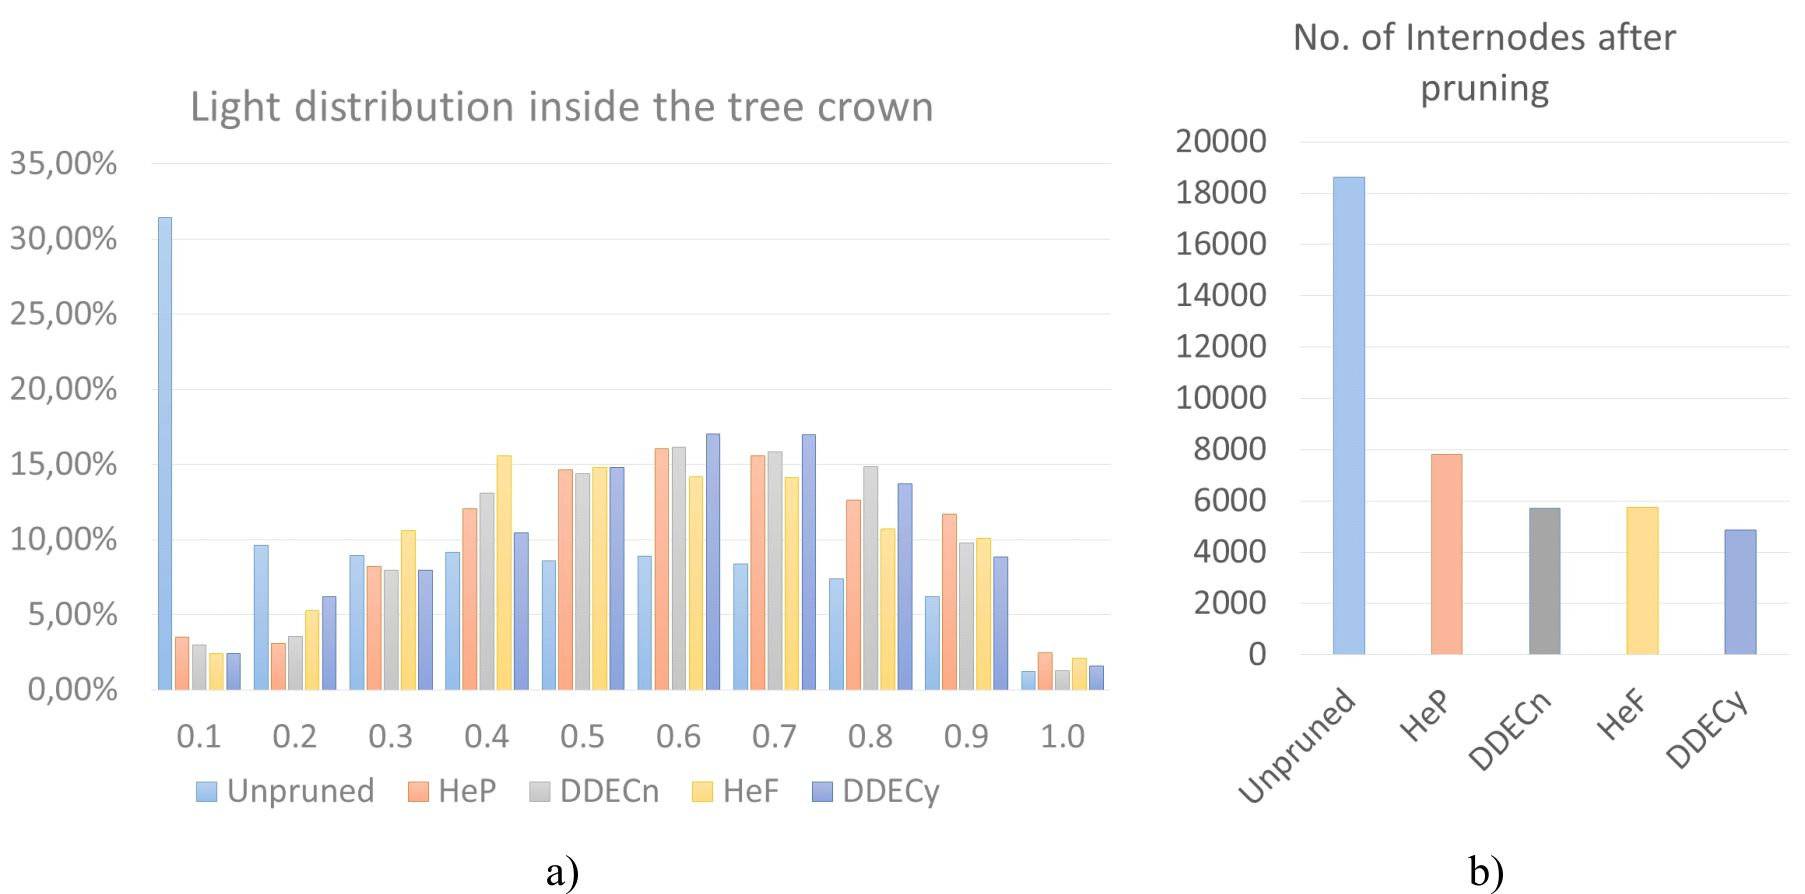
\includegraphics[width=\linewidth]{figs/image5.jpeg}
    \caption{Evaluation of tree pruning results, a) Comparison of
light distribution after the pruning by a human expert (HeP and HeF) and
automated pruning (DDECn and DDECy), b) Number of internodes left after
the pruning. A higher number of internodes, combined with higher light
exposure of buds signify better results.}
\label{fig:my_figure5}
\end{figure}

The DDECn and DDECy methods are representative of the selective pruning, where the
results of the first step represent the result of pruning by the
automatic pruning systems currently used. The difference between the
first and second step of DDECn and DDECy can be seen in Fig.~\ref{fig:my_figure6}. Visually, the trees after the second step are clearly less dense as the number of branches is drastically diminished,
while the overall height of the tree remains the same.

\begin{figure}[hbt]
    \centering
    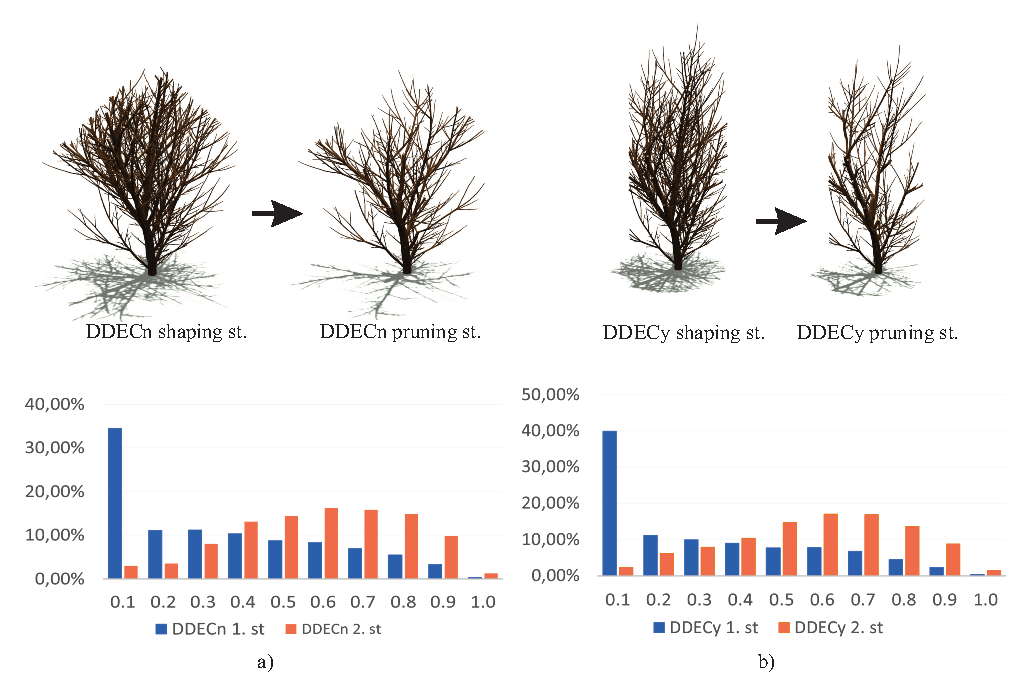
\includegraphics[width=\linewidth]{figs/Fig7.pdf}
    \caption{Tree crown light distribution after the shaping and
after the pruning step, a) DDECn method, b) DDECy method}
    \label{fig:my_figure6}
\end{figure}

\noindent\textbf{Long-term Pruning:} In another experiment, we evaluated a
long-term exposure to pruning. We were curious if the proposed automated tree pruning method is capable of tree training (i.e., getting the tree into desired growing form) without human intervention. We have
simulated a row of five trees for six consecutive years. At the
beginning of each year, the trees were pruned by the DDECn method to shape
them into the Slender Spindle growing form. The starting cone height was
1m and was linearly increased to 2.5m, which was the target height for
the trees in the following three years. The opening angle was constant
at $45^\circ$ for the experiment duration. The initial value of the parameter
\(s_{\mathrm{\max}}=20\) and was linearly increased to \(s_{\mathrm{\max}}=70\) in
the sixth year. The result of the experiment can be seen in Fig.~\ref{fig:my_figure7}.

As the tree structure becomes more complex in time, the
value of \(s_{\mathrm{\max}}\ \) should be increased. In our experiments
we observed that \(s_{\mathrm{\max}}\leq{150}\) even
for older trees provides reasonable results.
\begin{figure}[hbt]
    \centering
    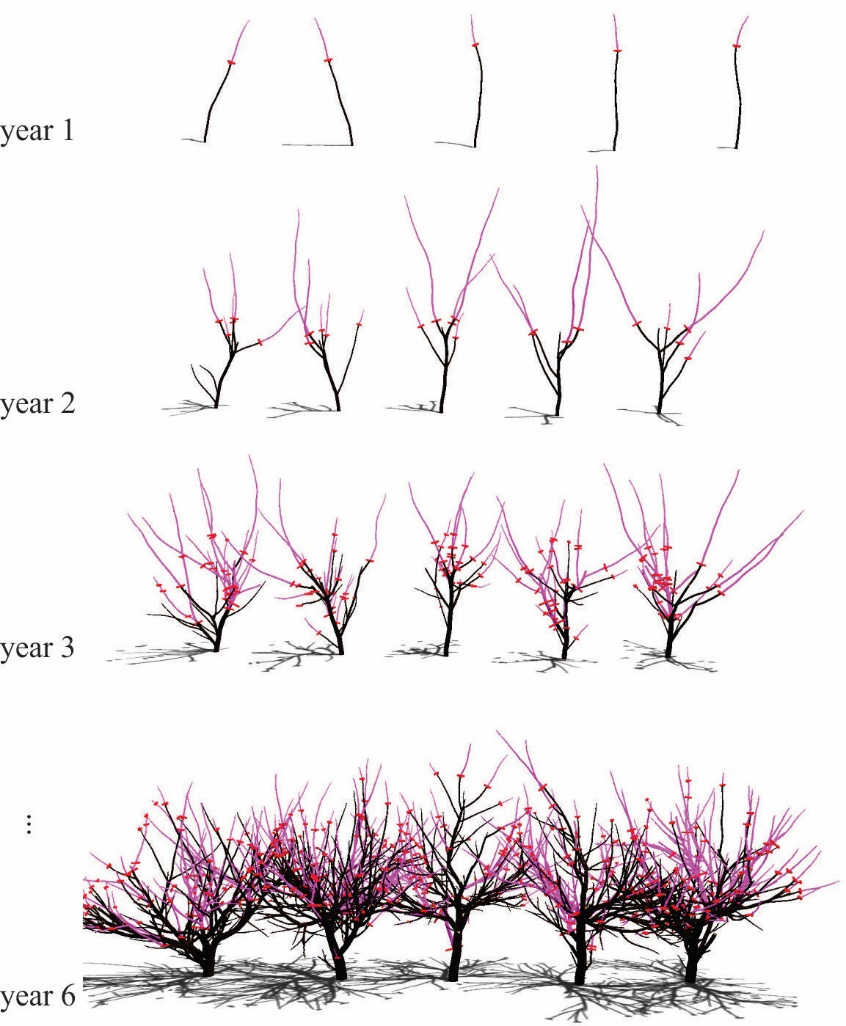
\includegraphics[width=0.8\linewidth]{figs/image7.jpeg}
    \caption{Tree training of five apple trees into a Slender
Spindle growing form for six consecutive years with the DDECn method.
The purple color denotes the branches removed at the pruning}
    \label{fig:my_figure7}
\end{figure}



\section{Conclusions and Future Work}
We have introduced an automated method for simulation of pruning of
trees and tree colonies. The objective was to propose pruning that
maximizes light exposure of buds within the crown and we used two step
method, where first step prunes the tree to a desired shape, and the
second step maximizes the bud irradiance. Our results show that our algorithm achieves results comparable
to the human pruning regarding the light
distribution inside the tree crown. The pruning simulation of a group of
trees for several consecutive years showed that the method could also be
used for the tree training towards desirable growing form. Since DDE is
a stochastic method, the set of excess branches that have to be removed
can vary from simulation to simulation. The solutions are not always
equally successful with respect to tree light crown distribution, but
the same is also true by the pruning solutions proposed by human pruning
expert.

The possible limitation of the proposed method is its strong dependency
on the tree growth model topological structure. This is important
because the challenging step in the automated tree pruning is the
construction of the appropriate tree model from tree images. Successful
algorithms of this kind are presented e.g, in~\cite{akbar_novel_2016,benes_visual_1997,de_reffye_plant_1988,palubicki_self-organizing_2009}.
However, they are not directly compatible with the EduAPPLE tree growth model and a
it would be important to bring these algorithms to a common ground, 
for example by generating the same tree representation. The construction of such representation would be even more desirable since the proposed pruning method shows pruning results comparable to human
expert. Some
work in this direction has already been done~\cite{kohek_estimation_2017}, 
but it is too early to assess its efficiency.

The main contribution of our work is to show that good pruning results
can be obtained automatically and without a fixed set of pruning rules.
This is not surprising since the pruning rules were developed by the
long-term experiments whose goal was to improve yield quality as well as
its quantity. Once the main parameters that influence the yield were
determined, the pruning techniques have been developed that maximize the
influence of those parameters and that is what the DDE objective
function is trying to mimic. Since light exposure is a critical
factor, the proposed method searched for the combination of cuts that
maximize the light exposure. This resulted in the higher light
distribution inside the tree crown. This distribution was also used for
evaluation of tree pruning since the obtained tree forms cannot be
compared directly. While the shapes of the trees in Fig.~\ref{fig:my_figure4} differ,
their light distributions are comparable. An additional pruning
benchmark is the number of internodes that corresponds to to the tree volume. 
The amount of removed internodes represents  the
pruning intensity and Fig.~\ref{fig:my_figure5}~b shows that the human expert preferred
slightly less aggressive pruning than the proposed method. The pruning
intensity by the proposed automated pruning is controlled by the
relation between tree volume and the value of the \(s_{\mathrm{\max}}\)
parameter. In order to preserve the tree pruning intensity, as the tree
is growing, the value of \(s_{\mathrm{\max}}\) should increase with the
increasing number of internodes in the tree. In our experiments, \(s_{\mathrm{\max}}=20\)
turned out to be the good initial value.

There are many possible avenues for future work. As mentioned above, coupling our method with other 
plant growth algorithms would be an important task to do. Another future work would be to use different optimization methods than the DDE. The long-term effect of growth should also be evaluated. It may be possible that the immediate value of bud illumination is not the most indicative factor and long-term plant health and development should be tested. Last but not least, our algorithm is a first step in an exciting direction of automated pruning. It would be interesting to automatically prune thousands of tree models and calculate statistics of the values we reported in Tables~\ref{tab:light} and~\ref{tab:inodes}. Although, we paid attention to report representative models, there may be a strong variation and statistics would provide a better representative value.
\section*{Acknowledgment}

The authors acknowledge the Project BI-US/17-18-012, and Programme
P2-0041 were supported financially by the Slovenian Research Agency.

\section*{Bibliography}
\bibliography{Bilateral}
\end{document}
